\section{Predobrada podataka i izbor atributa}
\label{ch:ch3}

\subsection{Predobrada}
Za predobradu podataka korišten je programski jezik Python u kombinaciji sa paketom Pandas. Datoteka s podacima \textit{splice\_orig.csv} je učitana u Pandas DataFrame objekt te su dodani nazivi atributa: \textit{class}, \textit{id} i \textit{dna} (vidi Tablicu \ref{tab:dataorig}).
\begin{table}[!ht]
   \caption[Primjeri instanci iz originalnog podataka]{
   \textbf{Primjeri instanci iz skupa podataka za dubinsku analizu} \textit{}}
   \centering
   \begin{tabular}{||c | c | c ||}
   \hline
   class & id & dna \\ [0.5ex]
   \hline\hline
   EI & ATRINS-DONOR-905 & AGACCCGCCGGGAGGCGGAGGACCTGC... \\
   EI & BABAPOE-DONOR-30 & GAGGTGAAGGACGTCCTTCCCCAGGAG... \\
   EI & CHPIGECA-DONOR-378 & CAGACTGGGTGGACAACAAAACCTTCA... \\
   .. & .. & .. \\
   N & ORAHBG2F-NEG-181  & ATCAATAAGCTCCTAGTCCAGACGCCAT... \\
   N & ORARGIT-NEG-241 & TCTCGGGGGCGGCCGGCGCGGCGGGG... \\
   N & TARHBD-NEG-1981  & AGGCTGCCTATCAGAAGGTGGTGGCTG... \\ [1ex]
   \hline
   \end{tabular}
   \label{tab:dataorig}
\end{table}

Nakon što smo izbacili stupac \textit{id} i podijelili stupac \textit{dna} podaci imaju oblik kao u tablici \ref{tab:datasplit}.

\begin{table}[!ht]
   \caption[Primjeri instanci iz procesiranog skupa podataka]{
   \textbf{Primjeri instanci iz procesiranog skupa skupa podataka za dubinsku analizu} \textit{
Stupac \textit{id} je jedinstveni identifikator vrste za svaki red u tablici i zbog toga ga ne koristimo u analizi podataka. Stupac \textit{DNA} dijelimo na šezdeset stupaca, za svaki nukleotid u DNA nizu po jedan novi stupac, naziva dna\_x gdje x označava indeks nukleotida u originalnom nizu.
   }}
   \centering
   \begin{tabular}{||c | c | c |c | c | c | c ||}
   \hline
   class & dna{\_1} & dna{\_}2 & dna{\_}3\ & dna{\_}4\ & dna{\_}5 & ...\\ [0.5ex]
   \hline\hline
   EI & A & G & A & C & C & ... \\
   EI & G & A & G & G & T & ... \\
   EI & C & A & G & A & C & ... \\
   .. & .. & .. & .. & .. & .. & ... \\
   N & A  & T & C & A & A & ... \\
   N & T  & C & T & C & G & ... \\
   N & A  & G & G & C & T & ... \\ [1ex]
   \hline
   \end{tabular}
   \label{tab:datasplit}
\end{table}

\begin{table}[!ht]
   \caption[Udjeli nukleotida u skupu podataka za dubinsku analizu]{
   \textbf{Udjeli nukleotida u skupu podataka za dubinsku analizu.} \textit{A, G, C i T čine značajnu većinu u skupu podataka. D, N, S i R čine neznatan dio skupa.}}
   \centering
   \begin{tabular}{||c | c | c ||}
   \hline
   Oznaka atributa & Broj atributa & Udio atributa (\%) \\ [0.5ex]
   \hline\hline
   A & 44475 & 23.244 \\
   T & 46298 & 24.196 \\
   G & 50226 & 26.249 \\
   C & 50281 & 26.278 \\
   D & 2  & 0.0010 \\
   N & 56 & 0.0293 \\
   S & 1  & 0.0005 \\
   R & 1  & 0.0005 \\ [1ex]
   \hline
   \end{tabular}
   \label{tab:udjeli}
\end{table}
Tablica \ref{tab:udjeli} pokazuje razdiobu jedinstvenih oznaka nukleotida. Vidimo da vrlo mali udio ima oznaku D, N, S ili R (ukupno 15 redaka). Zbog toga možemo izbaciti ove retke bez značajnog smanjenja skupa podataka za dubinsku analizu. S druge strane, na ovaj način sprječavamo da algoritam da previše važnosti podacima koji spadaju u ovu marginalnu skupinu (eng. \textit{outliers}). 
Jedna od instanci iz klase EI\footnote{HUMALPI1-DONOR} ima nukleotidni niz\textit{ 
ACACAGGGCACCCCCTCANNNNNNNNNNNNNNNNNNNNNNNNNNNNNNNNNNNNNNNNN
}. Čak 42 baze označene su s oznakom N. Ako bi svaki N zamijenili s jednom od četiri moguće baze dobili bismo 4\textsuperscript{42} kombinacija. Bez provjere u postojećim bazama podataka ne možemo znati koje su od tih kombinacija uistinu dijelovi donorskih sekcija u genomu. Korištenjem ovih kombinacija značajno bismo utjecali na distribuciju skupa podataka jer većina lokacija u genomima nije ni donorska ni akceptorska sekcija gena. 
Ovako obrađen skup podatak spremljen je u datoteku \textit{splice\_filtered.csv}

\subsection{Vizualizacija atributa}
Budući da su svi podaci u skupu nominalni, te da imamo veliki broj atributa, moguće ih je prikazati samo indirektnom mjerom ili parcijalno.

Prije nego krenemo s procesom obrade podataka dijelimo skup na dva dijela: skup za trening i skup za testiranje. Za testiranje izdvajamo 20\% od ukupnog skupa podataka i njih koristimo samo za završnu ocjenu odabranih trening algoritama. Funkcija \textit{test{\_}train{\_}split} iz modula model{\_}selection. Želimo osigurati da su podaci stratificirani, odnosno da su razdiobe podataka jednake u ishodišnom skupu podataka kao i generiranim skupovima. 
\begin{center}
   \begin{figure}[ht!]
      \begin{center}
         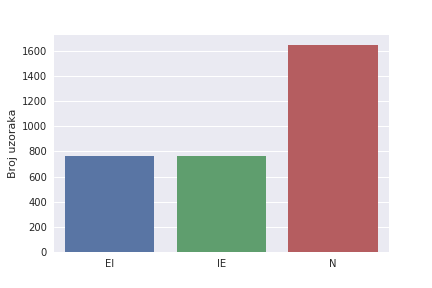
\includegraphics[height=5cm, width=8cm]{dataset_class_dist}
         \caption[Distribucija instanci u skupu podataka]
         {\textbf{Distribucija instanci u skupu podataka po klasama.}\textit{Prevladava klasa N, odnosno nizovi koji ne pripadaju ni akceptorskim ni donorskim nizovima nukleotida. U pojedinačnom genomu ova razlika je još izraženija\cite{Brown01} i kada bismo htjeli koristiti ovaj algoritam na drugim skupovima podataka morali bismo prilagoditi broj instanci odgovarajućim omjerima.}}
         \label{fig:dist_orig}
      \end{center}
   \end{figure}
\end{center}

Metoda \textit{test{\_}train{\_}split} ima argument \textit{stratify} kojem predajemo stupac s klasama. Slike \ref{fig:dist_orig} i \ref{fig:dist_train_test} potvrđuju da su podaci pravilno podijeljeni.

\begin{center}
   \begin{figure}[ht!]
   \begin{subfigure}{.5\textwidth}
         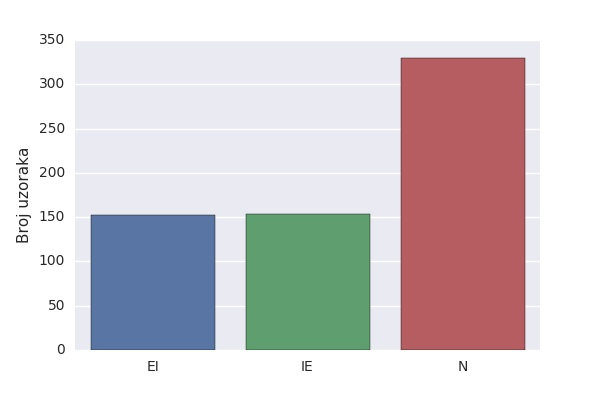
\includegraphics[height=5cm, width=7cm]{testset_class_dist}
         \caption{Trening}
         \label{fig:dist_train}
   \end{subfigure}
   \begin{subfigure}{.5\textwidth}
         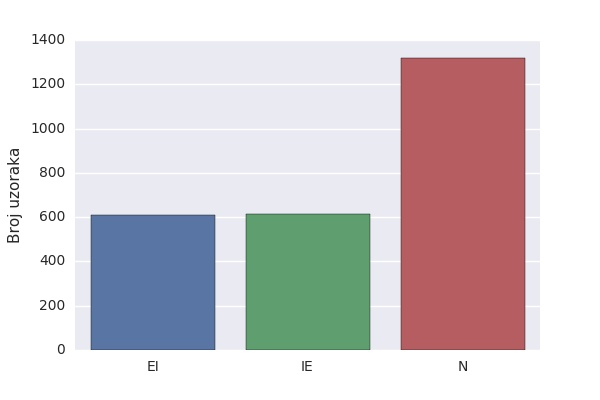
\includegraphics[height=5cm, width=7cm]{trainset_class_dist}
         \caption{Test}
         \label{fig:dist_test}
   \end{subfigure}
   \caption[Distribucija instanci u trening i testnom skupu podataka]
   {\textbf{Distribucija instanci u podijeljenim skupovima podataka po klasama.}\textit{Vidimo da je distribucija skupa za trening (a) i skupa za testiranje (b) jednaka distribuciji izvornog skupa podataka. Razlika je samo ukupnom broju instanci u pojedinome skupu.}}
    \label{fig:dist_train_test}
   \end{figure}
\end{center}

\subsection{Odabir atributa}
Pri kreiranju modela za dubinsku analizu podataka obično nije nužno koristiti sve dostupne atribute skupa podataka. U odabiru najboljih atributa za model primjenjuju se različite tehnike koje se u grubo mogu svrstati u tri kategorije. Metode \textbf{filtriranja} koriste najčešće različite statističke testove kako bi se odredila korelacija\footnote{termin korelacija ovdje koristimo u širem smislu, ne isključivo u statističkom kontekstu} između atributa i izlazne varijable (klase). Druga kategorija, metode\textbf{omotača}\footnote{eng. \textit{wrapper methods}} koriste se podskup atributa nad kojim treniraju model. Na osnovu zaključaka iz ovog modela, dodaju se ili oduzimaju određeni atributi - problem odabira atributa svodi se na problem pretraživanja. \textbf{Ugradbene} metode\footnote{eng. \textit{embedded methods}} kombiniraju kvalitete filterskih i metoda omotavanja korištenjem algoritama koji imaju vlastite ugrađene metode selekcije atributa.

Algoritam stabla odlučivanja ima prirodno ugrađen mehanizam za odabir atributa. Najprije se u postupku konstrukcije rangiraju atributi, a zatim se u postupku podrezivanja smanjuje ukupan broj atributa. Neki računalni znanstvenici\cite{Grabczewski01} zbog ovih karakteristika koriste stablo odlučivanja kao algoritam za odabir atributa koji će se zatim koristiti u drugom modelu (klasifikacija iili regresijski postupak). Budući da je procedura izgradnje stabla odlučivanja poprilično brza onda je moguće i koristiti sve atribute. Međutim, kako bi provjerili ovu hipotezu, kreirat ćemo i dodatne varijante stabla odlučivanja, nad atributima koje odaberemo pomoću Hi-Kvadrat testa.
\subsubsection{Hi-Kvadrat test}
Hi-Kvadrat je test nezavisnosti koji se koristi kako bi se odredilo postoji li značajna veza između dvije nominalne (kategorične) varijable. Frekvencija svake vrijednosti jedne nominalne varijable uspoređuju se sa kategorijama druge nominalne varijable. Nul-hipoteza 
